%% ==============
\chapter{Evaluation}
\label{ch:Evaluation}
%% ==============
In this chapter we compare all the techniques we implemented with plain uniform and powerbased Next Event Estimation and PBRTs implementation. We try to point out the strength and weaknesses of the techniques for certain kind of scenes and scenarios. In this context we mainly argue about image quality, time and memory. We compare time and momery consumtion based on the Mean Squared Error (MSE) metric from equation~\ref{eq:mse}. Where $Y_i$ is the vector of pixels of length $n$ of our reference image and $\widetilde{Y}_i$ is the vector of pixels of the compared image. 

\begin{align}\label{eq:mse}
\text{MSE} = \frac{1}{n}\sum_{i=1}^{n}\abs{Y_i - \widetilde{Y}_i}^2
\end{align}
\begin{align}\label{eq:rmse}
\text{RMSE} = \sqrt{\text{MSE}}
\end{align}


We compare based on an equal MSE, therefor the MSE is an estimator for our image quality. When we argue about image quality throughout this chapter we rather refer to the perceived image quality\footnote{The MSE in itself has a perception compontent because of the square. The MSE is a very commonly used estimator, nonetheless one could imagine using a metric which does reflect human perception more closely. This usually leads to problems with subjectivity.}, in our case this usually means whether sensible artifacts are present. As all the compared techniques are unbiased, given unlimited time, all of them would converge to the same image. Artifacts are usually areas or edges which will converge very slowly, in practice maybe never. When we say a technique has a bad image quality, we say that artifacts are present. 

\begin{align}\label{eq:sigmaCor}
\sigma \sim \frac{1}{\sqrt{N}}
\end{align}

...

\begin{figure}
\centering
\begin{subfigure}[b]{1\textwidth}
   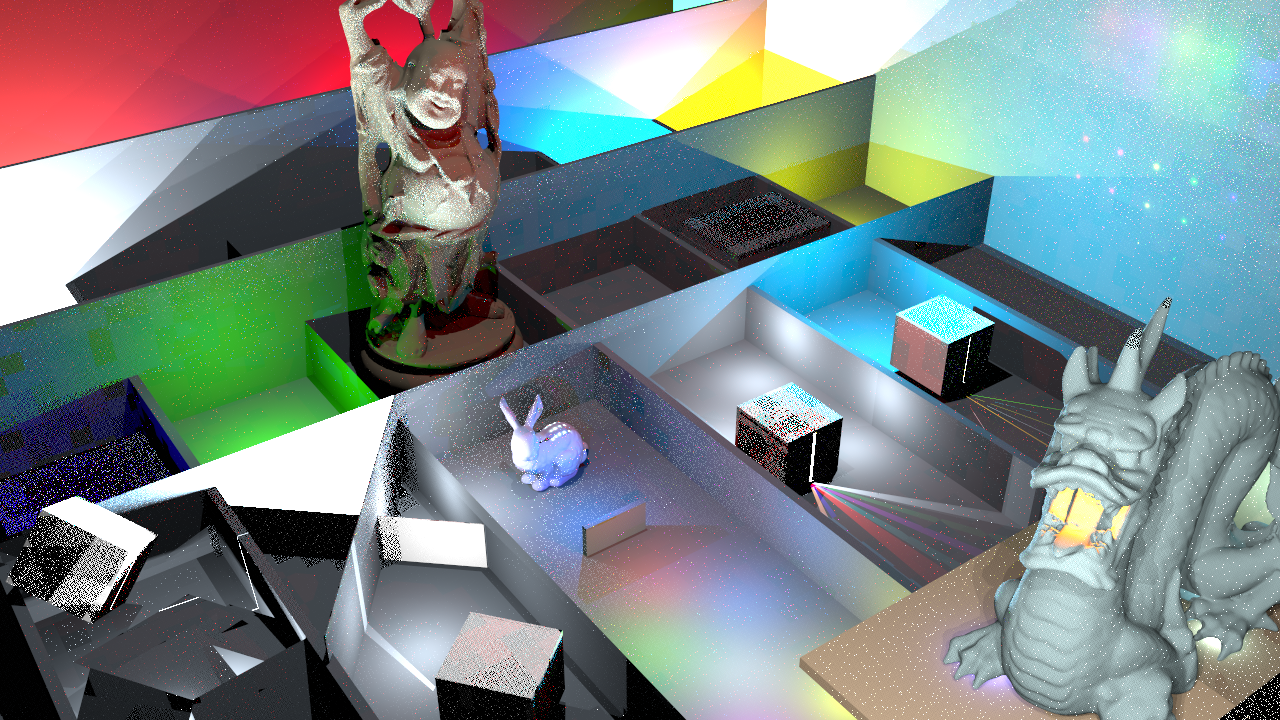
\includegraphics[width=1\linewidth]{figures/examples/StanfordMuseum_pvox_ps512_t503_icdf-0_pc96000k_mc0,1_Vox96_8854.png}
   \caption{Stanford-Museum rendered with 512 samples per pixel with \textit{cdfgrid} and no interpolation.}
   \label{fig:SMnoInt} 
\end{subfigure}

\begin{subfigure}[b]{1\textwidth}
   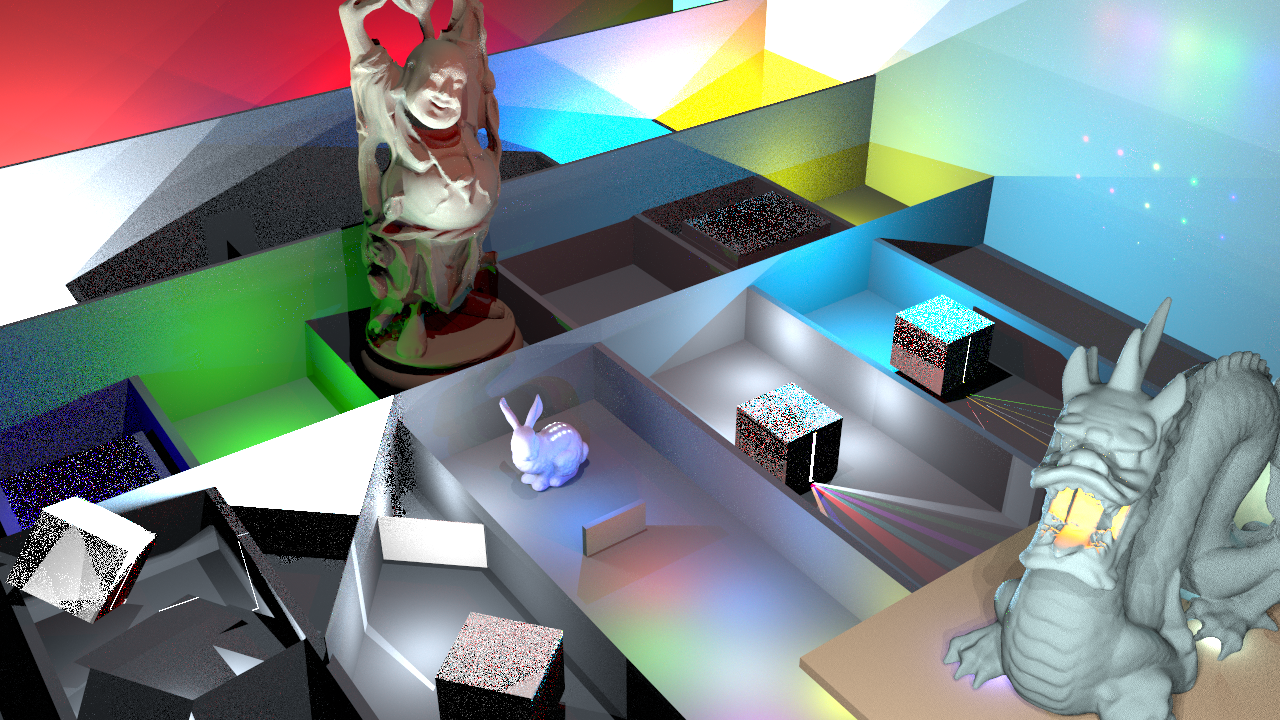
\includegraphics[width=1\linewidth]{figures/examples/StanfordMuseum_pvox_ps512_t723_icdf-1_pc128000k_mc0,1_Vox64_17574.png}
   \caption{Stanford-Museum rendered with 512 samples per pixel with \textit{cdfgrid} and trilinear interpolation.}
   \label{fig:SMInt}
\end{subfigure}

\caption{A visual comparison of no interpolation vs trilinear interpolation. Even though we already have a rather high sample per pixel count, (a) shows many clear variance edges of the underlying grid cells and various artifacts across the scene. Also it is remarkable how many fireflies are visible and how almost none of them are present in (b). It is quite apparent that a human observer would grade the image quality of (b) much higher, but surprisingly the RMSE of (a) is significantly smaller, $39.8$ versus $47.3$. The reason being, that aside of the fireflies and artifacts, the majority of pixels in (a) are less noisy. The difference in noise is less apparent at first, but is well illustrated on the white/gray wall to the left of the Buddah.}
\end{figure}


\section{Setup}

The test machine we use for comparisons is an Intel i7-4790K CPU @ 4GHz, 32 GB RAM, running on Windows 10 64-Bit. Images are produced by PBRT-v3, forked on March 30\footnote{Latest commit before the fork: \url{https://github.com/mmp/pbrt-v3/commit/42c42c194bab970d8adc3f6b5e3afbbc172c3375}}. PNEE techniques are added on top of this fork, the complete implementation can be found at \url{https://github.com/AndiMiko/pbrt-v3}.

\subsection{Problem cases}

We tried to identify problematic light and object constellations, which are causing trouble for various kinds of techniques. The most prominent and comprehensible scenarios are to be covered bellow. 

\begin{description}
    \item[1. High Frequency.] 
    \item[2. Level of Detail.]
    \item[3. High variantion of light power.] 
    \item[4. High number of contributing light sources.]
    \item[5. Non-axis aligned planes.]
    \item[6. Highly occluding planes.]
    \item[7. Tiny but important solid angles.]
\label{li:problemcases}
\end{description} 
% which problematic setups we have / we can solve

\subsection{Test scenes}

We designed a special scene, called \textit{Stanford-Museum}, for most of the comparisons we present in this chapter. This scene covers all aforementioned problem cases and thus gives a good impression about strengths and weaknesses of each technique. The simplicity of the scene allows the reader to clearly correlate variance with the problem cases, but ultimately does not provide a photorealistic appeal. On the other hand we present two more scenes, \textit{City} and \textit{measure-one}, for a comparison on real scenes with all sorts of details.

\paragraph{Stanford-Museum}

\begin{figure}[ht]\centering
\captionsetup[subfigure]{labelformat=empty}

\begin{tikzpicture}[zoomboxarray, zoomboxes below, zoomboxarray inner gap=0.4cm,
zoomboxarray columns=4, zoomboxarray rows=2,remember picture, black and white]
   \node [image node] {
   \setcounter{zoombox}{0} 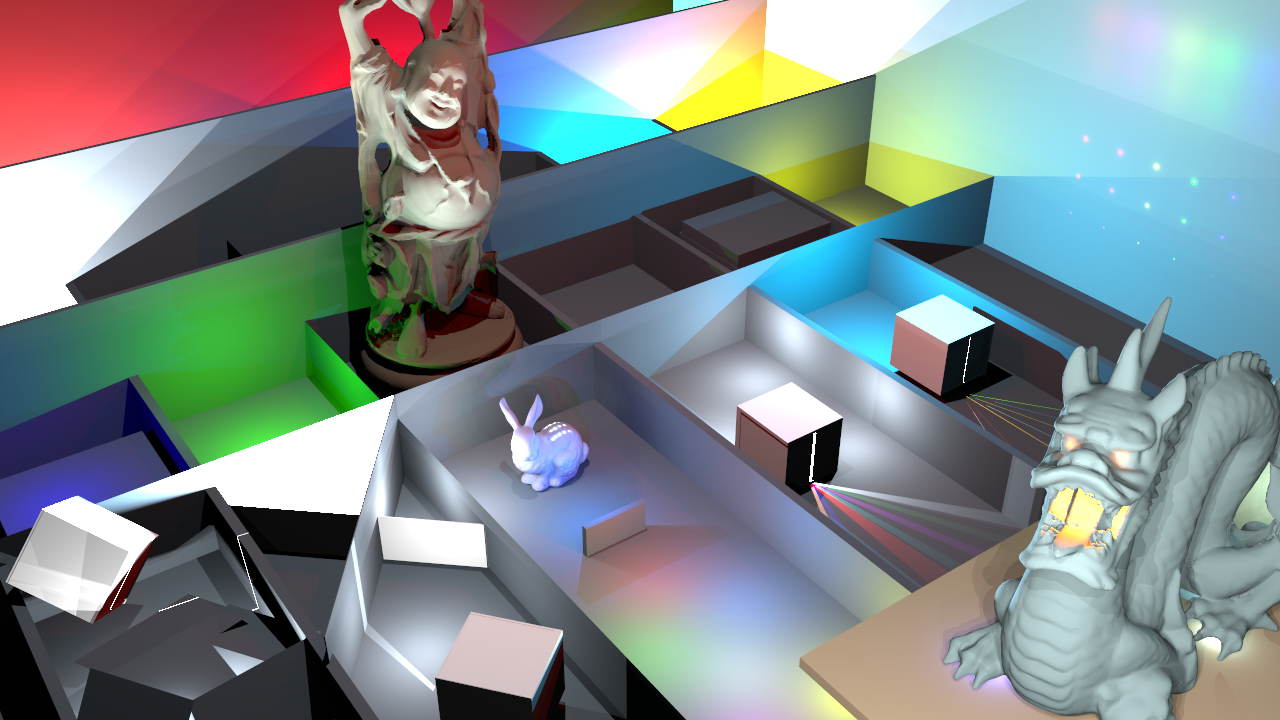
\includegraphics[width=1\textwidth]{figures/StanfordMuseum_ref.png}};
   
   \zoombox[magnification=0.8, color code=red]{0.85,0.3}
   \zoombox[magnification=1.5, color code=yellow]{0.334,0.78}
   
   \zoombox[magnification=2.3, color code=green]{0.767,0.47}
   \zoombox[magnification=1.4, color code=olive]{0.895,0.79}
   
   \zoombox[magnification=2, color code=brown]{0.285,0.32}
   \zoombox[magnification=1.3, color code=blue]{0.11,0.2}
   
   \zoombox[magnification=2, color code=cyan]{0.085,0.63}
   \zoombox[magnification=2, color code=pink]{0.6,0.68}

\end{tikzpicture}
\begin{tikzpicture}[overlay,remember picture]

\foreach \X in {1,...,\thezoombox}
   {\node[anchor=south,yshift=-13pt] at (zoombox-\X.south) 
   {\tiny (\X)};}
   \setcounter{zoombox}{0} 
\end{tikzpicture}

\caption{The reference image for \textit{Stanford-Museum} sampled with PBRTs directlighting integrator. Instead of NEE every light source is queried for any shading point. Max depth is one, thus no indirect illumination is present. All and more phenomenons from listing~\ref{li:problemcases} appear in this scene. Detailed descriptions and intentions of the zoomed areas are listed in~\ref{li:stanfordmuseum}.
}
\label{fig:stanfordmuseumref}
\end{figure}

We describe the most important problem cases we had in mind when designing the Stanford-Museum scene in figure~\ref{fig:stanfordmuseumref}, which is the reference image we calculate the MSE against. The scene contains 4058 light sources, all of whom are point light sources. We chose point light sources, because sampling a point on a area light source is not a concern of PNEE, thus reducing variance from other effects does discloses artifacts produced by our techniques more clearly. We also render the scene with a pathtracer with a max depth parameter of one, again, using the same argument, as depth introduces variance from the indirect lighting term of the pathtracer. Additionally, this makes rendering a nearly perfect reference image possible, by using PBRTs direct lighting integrator, which samples all point light sources for any intersection point. The reference image is rendered with 128 samples per pixel in 17 hours on our test machine. 

\begin{itemize}
    \item[(1)] The dragon is 20 times smaller than the Buddah but is very close to the camera and as such takes up almost the same screen space. Several low intensity point lights illuminate the dragon. The difference in size as well as light intensity constitute typical problem cases with LOD. Especially the illumination of the eyes is a rather extreme case, light source intensity is roughly 200.000 times less compared to the strongest light sources in the scene. Additionally, the left outline of the dragon is illuminated by various light sources from bellow in the scene, where the dragon takes up only an incredibly small solid angle and thus photons are very unlikely to hit the dragon.
    \item[(2)] The Buddah stands out of all cells and as such is illuminated by almost all visible light sources in this scene. This is particularly a problem for example with \textit{photontree}. There might be more light sources influencing a shading point, than the total number of nearest neighbors we collect. High geometric detail and blending of many light colors make the Buddah prone to fireflies.  All three Stanford models are also intended to add complexity for intersection tests to various parts of the scene. 
    \item[(3)] The box has a very tiny split from which is casts long range, very bright, very thin and high frequent light rays. Additionally, a lot of photons are stuck within the thin walled box, which highly complicates building good estimators with PNEE on the outside. Several more of this boxes with varying properties and surroundings are present in the scene. 
    \item[(4)] Similar to the Buddah this plane wall is illuminated by many light sources in the scene. Additionally, there is a matrix of point lights with varying brightness, distance and color. This variety has to be mapped to smooth transitions and high frequencies accordingly. Similar scenarios to this one do also appear in other parts of the scene, for example in front of the bunny, also with many smooth transitions, but where difficulties brought by global illumination are replaced with many local soft shadows. 
    \item[(5)] A cluster of roughly 1000 light sources. Only thin, non axis-aligned walls separates it from several distinct lightning scenarios. Very high exposure (unintentionally) breaks anti-aliasing. Most light sources influence the Buddah softly from bellow. 
    \item[(6)] Several non-axis aligned thin walls cover up a small cluster of light sources and cast thin, high frequent light rays in many directions. Especially the rays casted onto the scewed box, where photons from within the box, like mentioned in (3), do no good for our estimators, do constitute a tricky shading scenario in various manners.
    \item[(7)] Several strong light sources cast long range, smoothly fading, but sharp edged light rays. A similar scenario is present on the other side of the Buddah, where colors also blend together. The rays closely pass quite dark cells. Again, strong light sources behind a thin wall interfere with our photon collection algorithms.
    \item[(8)] A completely occluded light cluster with roughly 1000 light sources. In a real scene this might be a different room of a house for example. There are four such occluded clusters in the scene.
\label{li:stanfordmuseum}
\end{itemize}
\paragraph{Measure-one}




\paragraph{City}




\subsection{Techniques}

% which implementations will be compared

\subsection{Parameter Comparison}



%%%%%%%%%%%%%%%%%
\label{ch:ev:photontree}

%%%%%%%%%%%%%%%%%
\label{ch:ev:cdftree}

%%%%%%%%%%%%%%%%%%%%

\label{ch:ev:photonsampling}


%%%%%%%%%%%%%%%%%%%%%%%
\label{ch:ev:uniformfloor}

% which parameters did we try to configure. Which parameters turned out to be good and will be set as fixed?

\section{Equal time comparisons}

\section{Memory comparisons}

\section{Conclusions}
